% !TEX root = DesignDocument.tex

\section{File Conversion Testing}
\tab
    The file conversion was manually tested using a variety of inputs to ensure robust and consistent performance. As there are two libraries (assimp and FBX SDK), they were both manually tested for simple functionality as they were implemented. Manual tests included sending through file types that could be inputs for assimp and making sure that the files made it to the FBX section and output the correct file format (FBX). Some of the input file types tested included common and expect file types such such as STL, OBJ, DAE etc. Unsupported file types were also tested and appropriate errors from the conversion libraries were received. The file types supported by the system are available in Table \ref{tab:suportedfiletypes}. Large files were also tested to gauge how long the system could take to process files of different sizes. There are certain limitations on the HoloLens hardware regarding file size and complexity. Users are properly notified of these limitations by the HoloLens platform should they be an issue. The HoloLens limitations are not formerly noted here as they are already anticipated to change with future updates.  

    Files with embedded textures were also tested to ensure textures get converted with the file. With the file types tested, such as OBJ and FBX, the textures converted with the files as expected. The HoloLens default 3D file viewer does not currently support colors or textures, thus these features have not yet been able to be tested.

    Test files of varying complexity were gathered from a variety of sources to ensure maximum coverage by the Augmented Education platform. The following files comprised the original test group used to ensure proper conversion to a FBX format and rendering on the Microsoft HoloLens:
    \begin{itemize}
        \item An OBJ sphere generated in Maple.
        \item An FBX column provided by Dr. Brent Deschamp of SD Mines.
        \item An OBJ sine wave generated in Maple.
    \end{itemize} 
    
    A number of files of varying format type from \url{http://free3d.com} were also tested. These sample files included a car, building, spaceship, Batman, and other unique files. 
    
    Cheldon was also able to receive large sample architectural files in .fbx format from a relative. One architectural file rendered in the HoloLens, but the other two were too large to be supported by the device's current limitation for meshes and vertices able to be rendered in the viewer.

    Conversion examples can be seen in Figures \ref{Car-FBX}, \ref{Car-OBJ}, and \ref{Car-STL}.  
    
    In Figure \ref{Car-FBX}, a 3D model for a car in .fbx format was acquired. This file was used to test conversion to .obj format, the result of which can be seen in Figure \ref{Car-OBJ}. Figure \ref{Car-STL} is an STL file generated from the FBX file, using a DAE file as an intermediate format between the FBX SDK and assimp libraries. The STL file does not contain the colors or smooth surfaces that are present in the other file types, which is a limitation of the STL file format. This system works for converting STL $\rightarrow$ FBX as well, but the colors would not be present in the final file because that information is not contained in the STL. 
    
\begin{figure}[H]
    \centering
    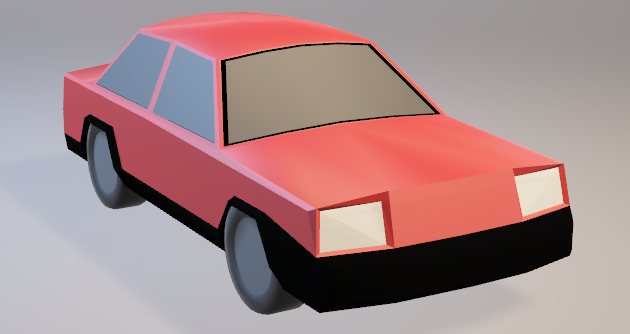
\includegraphics[width=\textwidth]{Car-FBX.png}
    \caption{Car FBX File}
    \label{Car-FBX}
\end{figure}

\begin{figure}[H]
    \centering
    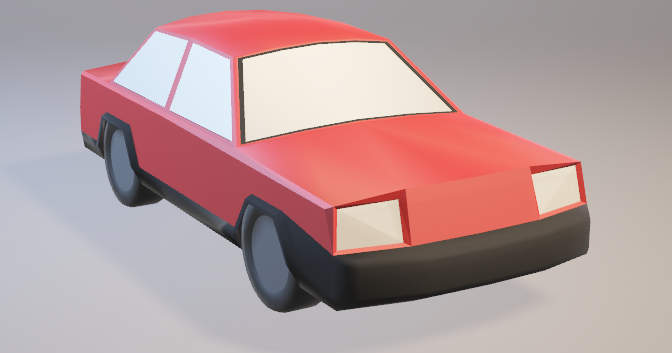
\includegraphics[width=\textwidth]{Car-OBJ.png}
    \caption{Car OBJ File}
    \label{Car-OBJ}
\end{figure}

\begin{figure}[H]
    \centering
    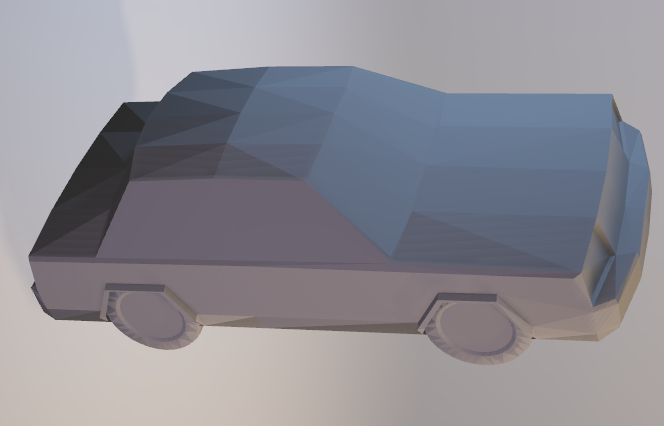
\includegraphics[width=\textwidth]{Car-STL.png}
    \caption{Car STL File}
    \label{Car-STL}
\end{figure}
